\documentclass[11pt]{article}
\usepackage[a4paper, left=3.17cm, right=3.17cm, top=2.54cm, bottom=2.54cm]{geometry}
\usepackage[fontset=mac]{ctex}
\usepackage[T1]{fontenc}
% \usepackage{mathtime}
% \usepackage{mathptmx}
\usepackage{amsfonts}
\usepackage{amsmath,amssymb,amsthm}
\usepackage{enumerate}
% 超链接
\usepackage{graphics}
% 算法描述的宏包
\usepackage[ruled]{algorithm2e}
\usepackage{algpseudocode,float}
\usepackage{lipsum}
\usepackage{chemformula}
\usepackage{cite}
\usepackage{subcaption}
\usepackage{booktabs}
\usepackage{multirow}
\usepackage{array}
% 超链接
\usepackage[colorlinks, linkcolor=black, anchorcolor=black, citecolor=black]{hyperref}
\usepackage{indentfirst}
\usepackage{graphicx}
\usepackage{cite}
\title{EvidentialMix:混合开闭集标签噪声的学习}
\author{Ragav Sachdeva,Filipe R. Cordeiro,Vasileios Belagiannis,\\ Ian Reid and Gustavo Carneiro}{}
\date{}
\makeatletter
\newenvironment{breakablealgorithm}
  {% \begin{breakablealgorithm}
   \begin{center}
     \refstepcounter{algorithm}% New algorithm
     \hrule height.8pt depth0pt \kern2pt% \@fs@pre for \@fs@ruled
     \renewcommand{\caption}[2][\relax]{% Make a new \caption
       {\raggedright\textbf{\ALG@name~\thealgorithm} ##2\par}%
       \ifx\relax##1\relax % #1 is \relax
         \addcontentsline{loa}{algorithm}{\protect\numberline{\thealgorithm}##2}%
       \else % #1 is not \relax
         \addcontentsline{loa}{algorithm}{\protect\numberline{\thealgorithm}##1}%
       \fi
       \kern2pt\hrule\kern2pt
     }
  }{% \end{breakablealgorithm}
     \kern2pt\hrule\relax% \@fs@post for \@fs@ruled
   \end{center}
  }
\makeatother

\begin{document}
\maketitle
\begin{abstract}
深度学习的有效性依赖于大规模的数据集,这些数据集是通过可靠而精心策划的数据
获取和标注过程得到的。然而,获取具有精确标注的大规模数据集是非常
昂贵和耗时的,而廉价的替代品通常会产生带有噪声标签的数据集。本文研究的领域通过
关注下面两种标签噪声的训练模型来解决这个问题:
1)闭集噪声,即一些训练样本被错误地标注为非真实类别的标签,但该标签在类别集合中;
2)开集噪声,即训练集包含的样本具有(严格地)不包含在已知训练标签集中的真实类别。
在本工作中,我们研究了一个标签噪声问题的变体,它结合了开集和闭集的标签噪声,
并引入了一个基准评价来评价在这个设定下训练算法的性能。
我们认为这样的问题更普遍 ,更好地体现了现实中噪声标签的场景。
此外,我们提出了一种新的算法,称为EvidentialMix, 
它解决了这个问题。我们将其性能与最先进的方法进行比较,设定为我们提出的在闭集和开集噪声上的基准。
结果表明我们的方法比最先进的模型产生了更好的分类结果和更好的特征表示。
我们的代码可以在如下的网址获取:\url{https:// github.com/ragavsachdeva/EvidentialMix}。
\end{abstract}
\newpage
\section{介绍}
深度学习利用大量且精心收集的训练数据,在几个重要的分类问题上取得了显著的结果[12,3]。
然而,社会中大多数感兴趣的数据集可用的数量级大而不容易收集,这意味着数据
可能包含获取和标记的错误,可以导致较差的泛化能力[26]。所以本邻域的一个重要的挑战
就是能够处理这种噪声标签数据集的方法的研发。 最近,研究人员极大地促进了这一领域的发展,
他们研究了受控的合成标签噪声,发现了可以应用于现实世界噪声数据集的理论或方法。

目前所研究的标签噪声类型可分为两类:闭集噪声和开集噪声。虽然这些术语(“闭集”和“开集”) 
是最近由wang等人在[24]中创造的,他们在论文中引入了有开集噪声的标签学习问题,
但闭集标签噪声问题已经被广泛地研究了很久。在处理闭集标签噪声时,大多数的学习算法假定
有一组固定的训练标签 [14,22]。在这个设定中,一些训练样本被标注到一个不正确的标签上,
而它们的真实类出现在训练标签集中。这些错误可以是完全随机的,即标签被任意地翻转到一个
不正确的类别上;也可以是一致的,如标注者确实对一个特定示例的标注感到困惑。
一个较少研究的标签噪声问题是开集噪声标签问题[24],其中我们错误地采样了一些数据,
导致它们的真实标注不包含在已知的训练标签集内。 这种设定的一个夸张的例子可能是:在用于
建模猫和狗的二分类问题中,训练集中出现一个马的图像。从他们的定义可以明显看出,
这两种标签噪声是互斥的,即一个给定的噪声标签不可能同时是闭集和开集。

很容易证明开放集和闭集噪声可能同时出现在真实世界的数据集中。
例如,最近的大规模数据收集方法提出使用查询商业搜索引擎获取数据(例如,谷歌图像检索)。其中搜索关键字
作为查询图像的标签。从图\ref{fig1}中可以看出,使用这种方法采集图像会导致同时存在开集噪声和闭集噪声。
然而到目前为止还没有关于混合标签噪声的系统研究,尽管已经有论文对他们提出的方法进行了
评估[13,24],但训练数据集被闭集噪声或开集噪声独立地破坏了,但从未被联合地破坏过。

\begin{figure}[h]
    \centering
    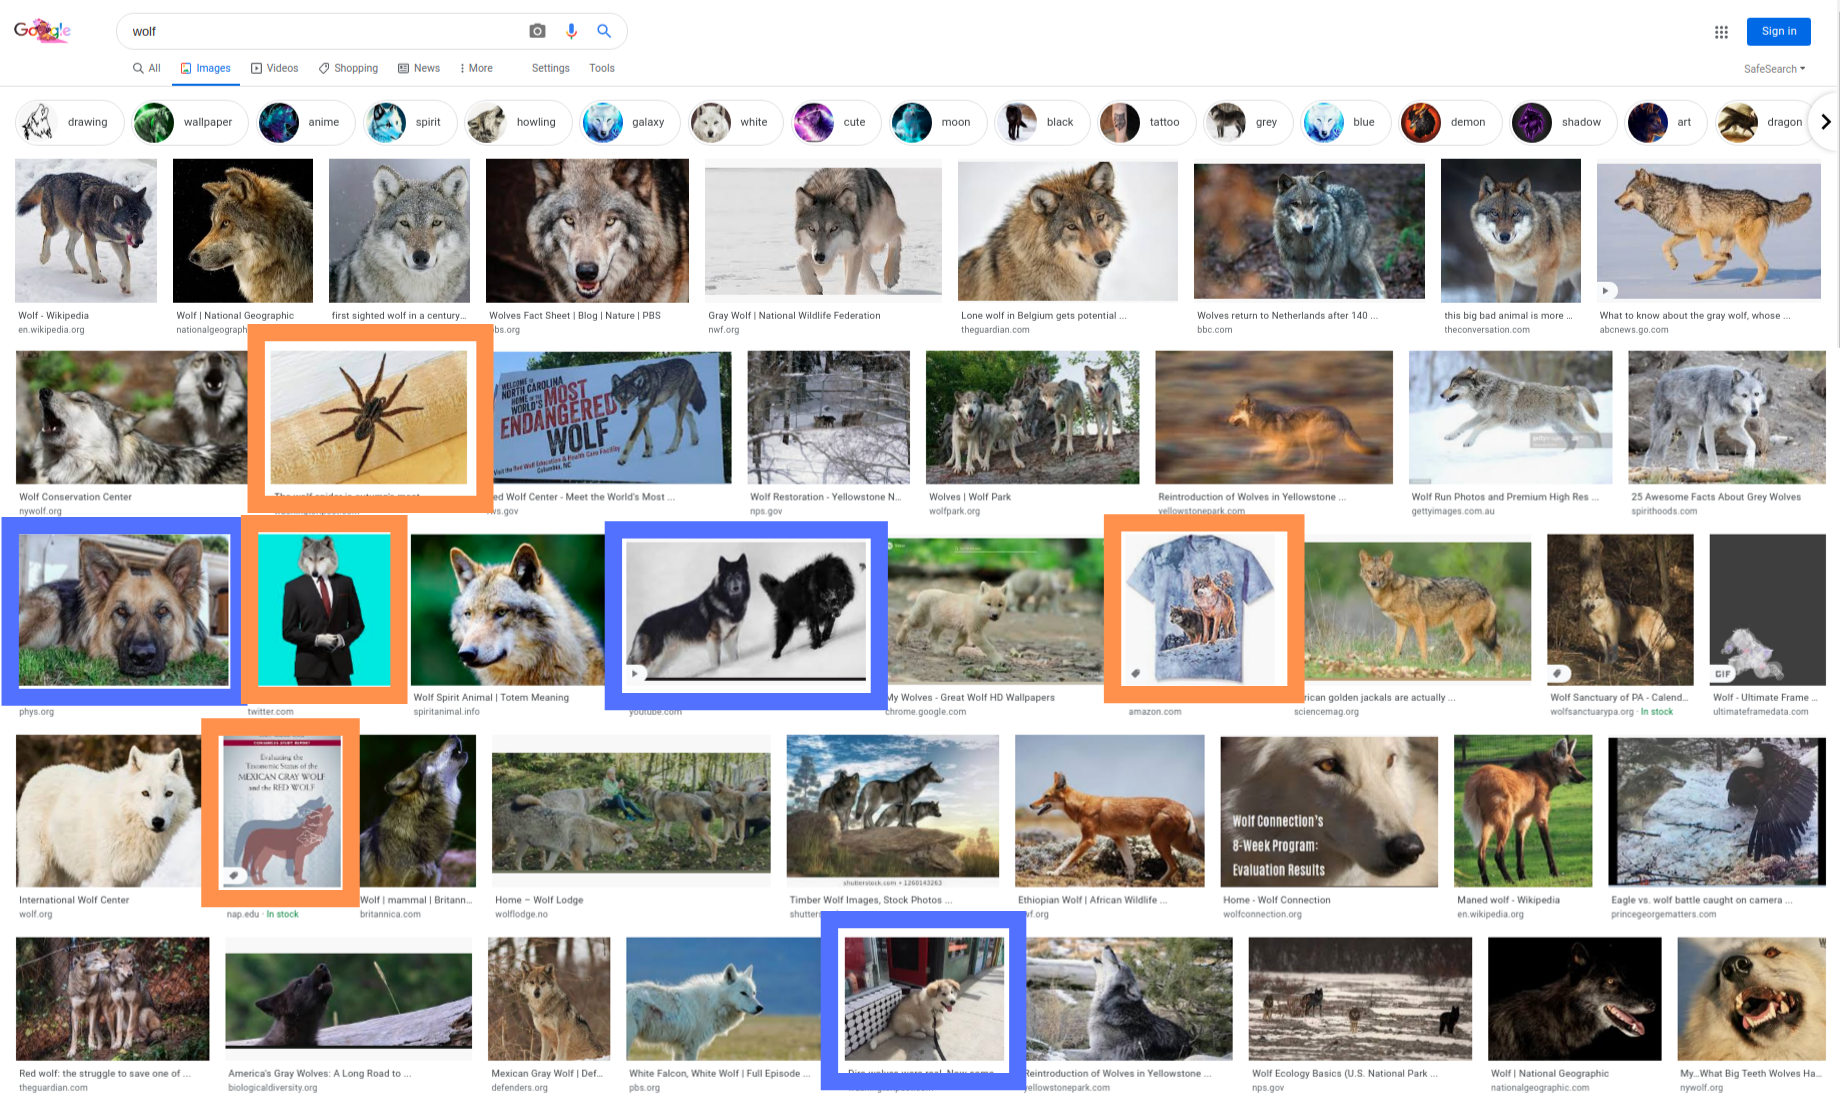
\includegraphics[width=0.8\textwidth]{images/wolfsearch.png}
    \caption{wolf-vs-dog二元分类器数据的搜索引擎查询结果。这里使用的搜索关键字是 “狼”。由一个橙色边框包围的图像是开集噪声样本 (即既不是狼也不是狗),被蓝色边框包围的是闭集噪声样本(即标签是狼,但实际上是狗)。}
    \label{fig1}
\end{figure}

在本文中,我们提出了一种新的基准评价来解决标签噪声学习问题,该问题由闭集噪声
和开集噪声的组合组成。这个提出的基准评估由三个变量定义:
1)标签噪声在训练集中所占的总比例,用$\rho \in [0,1]$表示;
2)标签噪声样本集中闭集标签噪声的比率,使用$\omega \in [0,1]$表示;
(这表示了整个训练集中有$\rho \times \omega $比例的样本含有闭集标签噪声,并且有
$\rho \times (1 - \omega) $比例的样本含有开集标签噪声)
3)开集噪声数据的来源。
注意这种设定同时是两种标签噪声的泛化。因为如果 $\omega \in \{0,1\}$,则样本可以被
破坏而具有其中的一种噪声。

最先进的(SOTA)方法旨在解决闭集噪声标签问题,其重点是识别不正确注释的样本,
并使用半监督学习(SSL)方法,更新它们的标签的[14]用于下一次训练迭代。这种策略
很可能在开集问题中失败,因为它假设每个训练样本的真实标签都在研究类别中存在,
但事实并非如此。 另一方面,解决开集噪声问题的主要方法[24]重点在学习过程中,
识别噪声样本并降低其权值。这种策略在闭集问题上效率很低 ,因为闭集的噪声样本在SSL阶段
仍然很有意义。因此,为了在存在闭集和开集噪声样本的情况下具有鲁棒性,
学习算法必须能够识别影响每个训练样本的标签噪声类型。根据类型,如果是闭集标签噪声样本,
则更新标签,如果是开集标签噪声样本则减少其权重。为了实现这一目标,我们提出了一种新的学习算法 ,
名为EvidentialMix (EDM),见图\ref{fig2}。我们提出的算法的关键贡献如下:
\begin{itemize}
    \item EDM能够准确区分干净的、开集和闭集噪声样本,从而允许它根据类型应用不同的
    学习机制。相比之下,以前的方法[14,24]只能将干净样本与噪声样本分离,
    而不能将闭集噪声与开集噪声样本分离。
    \item 我们发现我们的方法可以学习到比以前的研究方法更好的特征表示,如图\ref{fig4}
    中的t-SNE图所示,其中我们的方法对每个已知的标签/类都有一个唯一的聚类,
    而对开集样本给出另一个单独的聚类。相比之下,之前的方法显示出在开集样本上
    很大程度的过拟合,并错误地将它们聚到一个已知的类中。
    \item  我们的实验表明,EDM得到的分类精度,在不同的标签噪声率设定下(包括
    $\omega \in \{0,1\}$这样的极端情况)能够与之前的方法相媲美或能超过它们。
\end{itemize}
\begin{figure}[!htb]
    \centering
    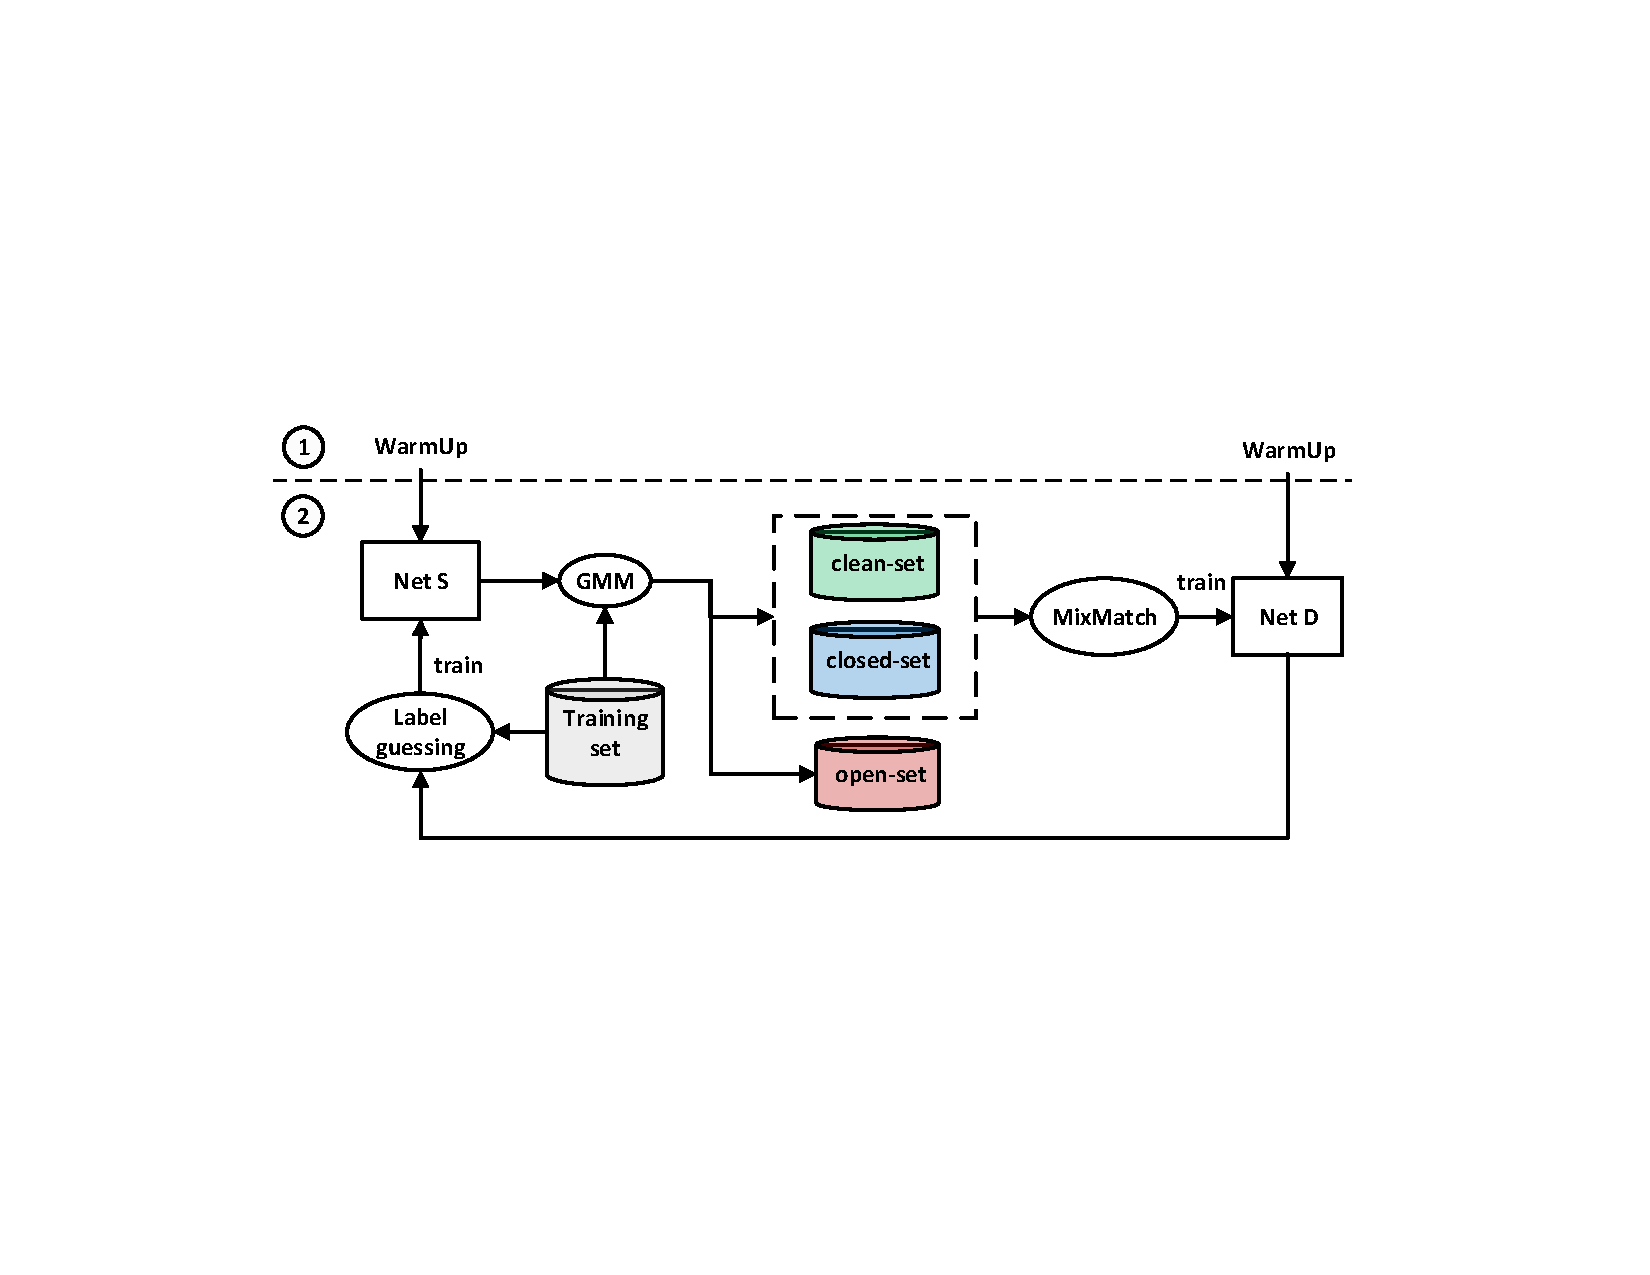
\includegraphics[width=0.8\textwidth]{images/diagrams/EDM_diagram_color6.pdf}
    \caption{我们提出的方法EvidentialMix依赖于两个
    网络,NetD和NetS。这两种模型最初都是使用一个简单的训练机制
    进行几个epoch(见(1)WarmUp)的训练,该机制不包含任何处理标签噪声的方法。接下来在
    (2)中,我们在NetS的样本损失上拟合一个$\psi$-分量高斯混合模型(GMM),以便将
    训练集分离为干净的、闭集和开集样本。在
    这之后,使用SSL学习机制[14]训练NetD,但只使用
    预测的干净和闭集样本。最后,NetS在整个训练集上进行
    训练,以使用NetD估计的标签最小化主观逻辑损失[21],并且
    (2)中的过程重复。}
    \label{fig2}
\end{figure}

\section{先前的研究}
人们对标签噪声设定下深度学习分类建模问题的研究越来越感兴趣。对于
闭集噪声,Reed 等人[19]提出了最早的方法之一,使用转移矩阵来表示标签如何在不同类别
之间切换。转移矩阵在不同的方法中被进一步探索[18,5],但它们都没有显示出有竞争力的结果,
可能是因为它们不包括识别和处理噪声样本的机制。数据增广方法[27]相继被
闭集标签噪声方法探索过,其思想是数据增广可以自然增加对噪声标签的训练鲁棒性。
元学习是另一种在闭集噪声标签问题中探索的技术[15,20],但由于需要干净的验证数据集或
人工的新训练任务,这项技术相对来说尚未被探索。研究者也探索了利用课程学习
(CL)[7]解决闭集噪声问题的方法,在训练过程中根据训练样本的损失值,动态地对训练样本
进行重新标记。该方法已经扩展成多模型训练方法[17,25],目的是聚焦到损失小的样本的训练上,
这些样本被多个模型不一致地分类。最近,Kim等人[9]研究了使用消极学习显式识别噪声样本,
获得了有竞争力的结果。另一种处理标签噪声的重要方法是Tarvainen等人[23]提出的模型集成。
利用具有鲁棒性的生成分类器(RoG)来提高判别分类器的性能的方法在Lee et al.[13]已经
进行了研究,他们从训练好的判别模型的几个层中提取特征,构建鲁棒的线性判别集成模型。
实际上,这种方法有可能提高任何方法的性能,并且已经接连在闭集和开集噪声场景中进行了测试。

开集标签噪声学习直到最近才被wang 等人[24]研究,其思想是识别出含有噪声标签的
样本,并在训练过程中减少它们的权重,因为它们几乎可以肯定属于一个不在训练标签集合中的
类别。鉴于他们的方法是唯一明确处理开集噪声的方法,他们的方法是解决开集标签噪声学习的
主要基准。

目前用于闭集标签噪声学习的SOTA方法是SELF[22]和DivideMix[14]——它们都结合了上述的
多种方法。SELF[22]结合了模型集成、重标记、噪声样本识别和数据增强;
而DivideMix[14]使用了多模型训练、噪声样本识别和数据增强[1]。这两种方法很容易
受到开集噪声的影响,因为它们假设训练样本必须属于某个训练类别——这个假设对于开集噪声来说
是不正确的。
\section{方法}
\subsection{问题定义}
我们定义训练集为$\mathcal{D}=\{(\mathbf{x}_i,\mathbf{y}_i)\}_{i=1}^{|\mathcal{D}|}$,
其中RGB图像为$\mathbf{x}:\Omega \rightarrow \mathbb{R}^3$ ($\Omega$ 表示图像晶格)。
训练标签集合用$\mathcal{Y}$表示,形成了$|\mathcal{Y}|$维度下的标准基,
$\mathbf{y} \in \{0,1\}^{|\mathcal{Y}|}$ ($\sum_{c=1}^{|\mathcal{Y}|}\mathbf{y}(c)=1$,
表示是一个多分类问题)。注意$\mathbf{y}_i$表示的是$\mathbf{x}_i$的噪声标签,潜在的
真实标签用$\mathbf{y}^{*}_i$表示。

对于\textbf{闭合标签噪声问题,噪声率}为$\zeta \in [0,1]$,我们假定
$(\mathbf{x}_i,\mathbf{y}_i) \in \mathcal{D}$以概率$1-\zeta$被标记为
$\mathbf{y}_i = \mathbf{y}^*_i$ ,并以$\zeta$概率被标记为$\mathbf{y}_i \sim r(\mathcal{Y})$,
$r(\mathcal{Y},\theta_r)$表示一个随机函数,从$\mathcal{Y}$选择一个标记,由一个特定
分布以及其参数$\theta_r$控制。

对于\textbf{开集标签噪声问题,噪声率}为$\eta \in [0,1]$,我们需要定义一个新的训练集
$\mathcal{D'}$(满足$\mathcal{D'} \cap \mathcal{D} = \emptyset$)。其中
$\mathcal{D'}$的标签集合用$\mathcal{Y'}$表示(满足$\mathcal{Y'} \cap \mathcal{Y} = \emptyset$)
——这意味着在$\mathcal{D'}$中的图像不再具有$\mathcal{Y}$中的标签。在这样的开集标签噪声学习问题中,
有$1-\eta$比例的样本从$(\mathbf{x}_i,\mathbf{y}_i) \in \mathcal{D}$且$\mathbf{y}_i=\mathbf{y}^{*}_i$的
样本中抽取。另外$\eta$比例的样本从$(\mathbf{x}_i,\mathbf{y}_i) \in \mathcal{D}'$且
$\mathbf{y}_i  \sim r(\mathcal{Y},\theta_r)$的样本中抽取。

对于\textbf{混合的开集和闭集标签噪声问题,噪声率}为$\rho,\omega \in [0,1]$,
混合了上述两种噪声定义。更具体地,$1 - \rho$比例的训练集包含图像$(\mathbf{x}_i,\mathbf{y}_i) \in \mathcal{D}$,标记为
$\mathbf{y}_i = \mathbf{y}_i^{*}$,然而$\omega \times \rho$比例的样本采样自
$(\mathbf{x}_i,\mathbf{y}_i) \in \mathcal{D}$,且标签为$\mathbf{y}_i  \sim r(\mathcal{Y},\theta_r)$。
$(1 - \omega) \times \rho$比例的样本来自集合$\mathcal{D}'$,
且被标记为$\mathbf{y}_i  \sim r(\mathcal{Y},\theta_r)$。

\subsection{噪声分类}
处理这个问题时的主要障碍是需要识别闭集和开集噪声样本,因为它们必须用不同的方法处理。
一种可能的方法是将闭集噪声样本与置信度高而分类错误时[14]计算出的高损失相关联,
将开集样本与不确定的分类相关联。为了实现这一点,我们使用了主观逻辑(SL)损失函数[21],
依赖于证据推理理论和SL来量化分类不确定性。SL损失利用Dirichlet分布来代表主观意见,
对信念和不确定性进行编码。使用SL损失进行训练的网络试图将预测后验的参数构成Dirichlet密度函数
进而对训练样本进行分类。对于给定样本的输出结果被认为是在一组类别标签上对该样本进行
分类的证据。图\ref{fig3}显示了使用SL损失训练的网络中样本的损失分布。很容易观察到干净、闭集
和开集噪声样本之间的区别。
\begin{figure}[h]
    \centering
    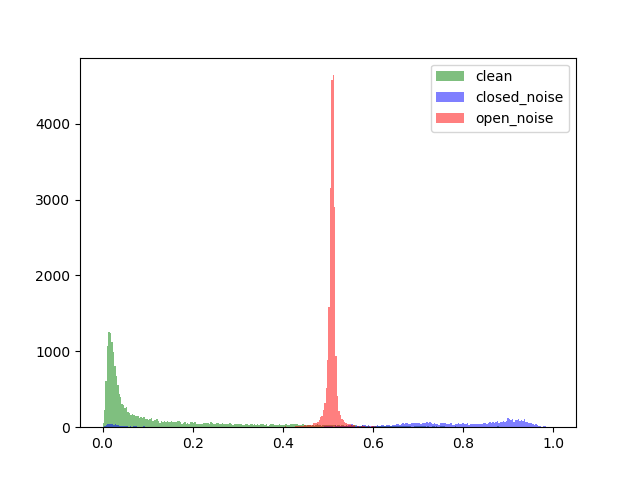
\includegraphics[width=0.5\textwidth]{images/textbook.png}
    \caption{预热阶段过后,使用SL损失函数时逐样本的损失分布。其中全部噪声比率$\rho = 0.6$,闭合噪声比率$\omega = 0.25$(也就是开集噪声比率为$1-\omega = 0.75$)。$\mathcal{D}$为CIFAR-10,$\mathcal{D}'$为ImageNet32。}
    \label{fig3}
\end{figure}
\subsection{EvidentialMix}
我们提出的EvidentialMix方法同时训练两个网络:使用SL损失[21]的NetS、
使用SSL训练机制和DivideMix(DM)损失[14]的NetD。广义地说,SL损失估计分类不确定性
的能力允许NetS将训练集划分为干净样本、开集和闭集噪声样本。预测的干净样本和闭集样本
随后被用来配合MixMatch(如[14]所述)训练NetD,而预测的开集噪声样本在当前周期被丢弃。
在此之后,NetD重新标记整个训练数据集(包括预测的开集样本),然后用来训练NetS。

随着NetS不断地从NetD预测的标签中学习,它可以更好地将数据分成三个集合。
这是因为NetD预测的标签在训练过程中变得更加准确,因为它只在干净样本和闭集样本上进行
训练,而从不训练被预测为开集的样本。这两个网络相互补充,从而对组合的闭集和开集噪声问题
产生准确的分类结果。下面列出了详细的解释,而算法\ref{alg:EDM}详细地描述了整个训练过程。

算法\ref{alg:EDM}训练NetD,通过$f_{\theta^{(D)}}(c|\mathbf{x})$表示,并且训练
NetS,通过$f_{\theta^{(S)}}(c|\mathbf{x})$表示(其中$c \in \{1,...,|\mathcal{Y}|\}$)。
——两个网络都可以得到$\mathbb R^{|\mathcal{Y}|}$空间的(logit)。在预热阶段(见WarmUp($\mathcal{D})$行),
我们在有限数量的周期内同时训练两个网络,其中对于$f_{\theta^{(D)}}(c|\mathbf{x})$的
训练使用交叉熵损失,此时概率通过Softmax激活函数$\sigma(.)$获得,形成
$p_{\theta^{(D)}}(c|\mathbf{x}) = \sigma(f_{\theta^{(D)}}(c|\mathbf{x}))$,
对于$f_{\theta^{(S)}}(c|\mathbf{x})$使用如下的SL损失:
\begin{equation}
    \mathcal{L}^{(S)} = \frac{1}{|\mathcal{D}|}\sum_{i=1}^{|\mathcal{D}|} \ell^{(S)}(\mathbf{x}_i,\mathbf{y}_i,\theta^{(S)}),
    \label{eq:S_loss}
\end{equation}

根据[21]:
\begin{equation}
    \ell^{(S)}(\mathbf{x}_i,\mathbf{y}_i,\theta^{(S)}) = \sum_{c = 1}^{|\mathcal{Y}|} (\mathbf{y}_i(c) - \alpha_{ic}/S_i)^2 + \frac{\alpha_{ic} (S_i - \alpha_{ic})}{S_i^2(S_i+1)},
    \label{eq:S_loss_sample}
\end{equation}

其中,对于每个类别$c \in \{1,...,|\mathcal{Y}|\}$,有$\alpha_{ic}=\varphi(f_{\theta^{(S)}}( c | \mathbf{x}_i)) + 1$ 。
$\varphi(.)$表示ReLU激活函数,且$S_i = \sum_{c = 1}^{|\mathcal{Y}|} \alpha_{ic}$。

对样本分类成干净、开集、闭集三个类别是通过公式\eqref{eq:S_loss_sample}对于整个训练集$\mathcal{D}$的SL损失实现的。
更具体地,我们使用了损失集合$\{ \ell^{(S)}(\mathbf{x}_i,\mathbf{y}_i,\theta^{(S)}) \}_{i=1}^{|\mathcal{D}|}$ 
并使用期望极大化算法(EM)拟合了一个$\psi$-分量的高斯混合模型(GMM)。我们在本文中探索
的想法在于,模型对\textbf{干净样本}的输出趋于自信,同时与原始标签一致,产生一个小的损失。模型对
\textbf{闭集噪声样本}的输出趋于自信但是同时和原始标签不一致,产生一个大的损失值。
然而,对于\textbf{开集噪声样本},模型将不会产生可信输出,导致损失值既不大也不小。因此,多分量
GMM模型将会捕获每个这些集合,得到样本分类为干净的概率 $w_i$,即后验概率
$p(\mathcal{G}|\ell^{(S)}(\mathbf{x}_i,\mathbf{y}_i,\theta^{(S)}))$。其中
$\mathcal{G}$表示均值$\leq \mu_{min}$的高斯分量的集合(也就是说小损失的分量集合)。
分类为闭集噪声样本的后验概率为$w_i^{\text{cl}}=p(\mathcal{G}^{\text{cl}}|\ell^{(S)}(\mathbf{x}_i,\mathbf{y}_i,\theta^{(S)}))$ ,
通过均值$\geq \mu_{max}$的高斯分量集合进行计算。

\newpage
\begin{algorithm}[H]
    \label{alg:EDM}
    \caption{EvidentialMix(EDM)}%算法名字
    \LinesNumbered %要求显示行号
    \KwIn{$\mathcal{D}=\{(\mathbf{x}_i,\mathbf{y}_i)\}_{i=1}^{|\mathcal{D}|}$, number of augmentations $M$, temperature sharpening $T$, loss weights $\lambda^{(\mathcal{U})}$ and $\lambda^{(reg)}$, MixMatch parameter $\alpha$, number of epochs $E$.}%输入参数
    \KwOut{output result}%输出
    $f_{\theta^{(D)}}(c|\mathbf{x}), f_{\theta^{(S)}}(c|\mathbf{x})$ = WarmUp($\mathcal{D}$)\;
    \While{$e < E$}{
  $\mathcal{W},\mathcal{W}^{\text{op}},\mathcal{W}^{\text{cl}}$ = GMM($\mathcal{D}, f_{\theta^{(S)}}(c|\mathbf{x})$) \\
  \tcp{Train NetD}
  $\mathcal{X} = \{ (\mathbf{x}_i, \mathbf{y}_i, w_i) | (\mathbf{x}_i, \mathbf{y}_i, w_i) \in (\mathcal{D},\mathcal{W}) , w_i >   \max(w_i^{\text{op}},w_i^{\text{cl}})\}$ \\  
  $\mathcal{U} = \{\mathbf{x}_i| (\mathbf{x}_i, \mathbf{y}_i) \in \mathcal{D} , w_i^{\text{cl}} >   
  \max(w_i,w_i^{\text{op}})\}$ \\
  \For{iter=1 \textbf{to} num\_iters}   
        {
            $\{(\mathbf{x}_b, \mathbf{y}_b, w_b)\}_{b=1}^{B} \subset \mathcal{X}$ \tcp{randomly pick $B$ samples from $\mathcal{X}$}
            
            $\{\mathbf{u}_b\}_{b=1}^{B} \subset \mathcal{U}$ \tcp{randomly pick $B$ samples from $\mathcal{U}$}
            
            \For{b=1 \textbf{to} B}   
            {
                \For{m=1 \textbf{to} M}   
                {
                    $\hat{\mathbf{x}}_{b,m}$ = DataAugment($\mathbf{x}_b$)  \\
                    $\hat{\mathbf{u}}_{b,m}$ = DataAugment($\mathbf{u}_b$) \\
                }
                \For{c=1 \textbf{to} $|\mathcal{Y}|$}
                {
                    $\mathbf{p}_b(c) = \frac{1}{M}\sum_m p_{\theta^{(D)}}(c|\hat{\mathbf{x}}_{b,m})$\\
                    $\mathbf{q}_b(c) = \frac{1}{M}\sum_m p_{\theta^{(D)}}(c | \hat{\mathbf{u}}_{b,m})$ \\
                }
                $\hat{\mathbf{y}}_b$ = TempSharpen$_{T}(w_b \mathbf{y}_b + (1-w_b)\mathbf{p}_b)$ \\
                $\hat{\mathbf{q}}_b$ = TempSharpen$_{T}(\mathbf{q}_b)$ \\
            }
            $\hat{\mathcal{X}} = \{(\hat{\mathbf{x}}_{b,m},\hat{\mathbf{y}}_b)\}_{b \in (1,...,B), m \in (1,...,M)}$ \\
            $\hat{\mathcal{U}} = \{(\hat{\mathbf{u}}_{b,m},\hat{\mathbf{q}}_b) \}_{b \in (1,...,B), m \in (1,...,M)}$ \\
            $\mathcal{X}', \mathcal{U}' = \text{MixMatch}_{\alpha}(\hat{\mathcal{X}},\hat{\mathcal{U}}$) \\
            $\theta^{(D)} = \text{SGD}(\mathcal{L}^{(D)},\theta^{(D)},\mathcal{X}', \mathcal{U}')$ \\
        }
        \tcp{Train NetS}
        \For{i=1 \textbf{to} $|\mathcal{D}|$}
        {
            $\hat{c}_i = \arg\max_{c \in \mathcal{Y}} \left [ (w_i^{\text{cl}}) p_{\theta^{(D)}}(c|\mathbf{x}_i) +
                (1-w_i^{\text{cl}}) \mathbf{y}_i(c)) \right ]$\\
            $\hat{\mathbf{y}}_i = \text{onehot}(\hat{c}_i) $\\
        }
        $\theta^{(S)} = SGD(\mathcal{L}^{(S)},\theta^{(S)},\{ (\mathbf{x}_i,\hat{\mathbf{y}}_i) \}_{i=1}^{|\mathcal{D}|}$) \\
 }
 
\end{algorithm}

\newpage
分类为开集噪声样本的概率则使用剩余的高斯分量进行计算,分量的均值$\in(\mu_{min},$  $\mu_{max})$ 
——这些后验概率形成了三个集合$\mathcal{W}=\{ w_i \}_{i=1}^{|\mathcal{D}|}$,
$\mathcal{W}^{\text{cl}}=\{ w^{\text{cl}}_i \}_{i=1}^{|\mathcal{D}|}$ 
和 $\mathcal{W}^{\text{op}}=\{ w^{\text{op}}_i \}_{i=1}^{|\mathcal{D}|}$。
使用这些后验概率,我们可以建立干净样本集,表示为$\mathcal{X}$,包含被预测为干净样本的
概率$w_i$大于其他两种类型的样本。同时建立闭合噪声样本集,表示为$\mathcal{U}$,包含被预测为
闭集标签噪声样本的概率$w_i^{\text{cl}}$大于其他两种类型的样本。

接下来,我们通过干净样本集$\mathcal{X}$和闭合噪声样本集$\mathcal{U}$训练NetD,样本集
在上文中已定义。一个小批次从$\mathcal{X}$和$\mathcal{U}$中抽取。此外,我们增广了每个
集合中的样本$M$次[14]。对于干净样本和闭集噪声样本的平均预测概率通过计算$M$次增广的平均值得到,
计算是在“温度尖锐化”之后进行的,通过TempSharpen$_T(.)$表示,其中 $T$表示温度。从而
对干净和闭集噪声样本形成“新”的样本和标签,分别为
$\hat{\mathcal{X}} = \{ (\hat{\mathbf{x}}_{b,m},\hat{\mathbf{y}}_b)\}_{b,m=1}^{B,M}$ 和
$\hat{\mathcal{U}} = \{ (\hat{\mathbf{u}}_{b,m},\hat{\mathbf{q}}_b)\}_{b,m=1}^{B,M}$
在随机梯度下降(SGD)的上一个阶段是MixMatch过程[1],其中$\hat{\mathcal{X}}$ 和 $\hat{\mathcal{U}}$
的样本是$\mathcal{X}'$ 和 $\mathcal{U}'$中样本的线性组合。SGD最小化DM损失,该损失融合了如下
的多种损失[14]:
\begin{equation}
    \mathcal{L}^{(D)} = \mathcal{L}^{(\mathcal{X})} + \lambda^{(\mathcal{U})}\mathcal{L}^{(\mathcal{U})} + \lambda^{(reg)}\mathcal{L}^{(reg)},
    \label{eq:D_loss_full}
\end{equation}
其中$\lambda^{(\mathcal{U})}$表示无标签样本集合的损失的权重,$\lambda^{(reg)}$表示
正则化项的权重。公式\eqref{eq:D_loss_full}中损失项的定义如下所示:
\begin{equation}
    \mathcal{L}^{(reg)} = \sum_{c=1}^{|\mathcal{Y}|} \frac{1}{|\mathcal{Y}|} \log \left ( \frac{1}{|\mathcal{X}'| + |\mathcal{U}'|} \sum_{\mathbf{x} \in (\mathcal{X}' \bigcup \mathcal{U}')} p_{\theta^{(D)}}(c|\mathbf{x}) \right ),
    \label{eq:L_reg}
\end{equation}

其中
\begin{equation}
    \begin{split}
        \mathcal{L}^{(\mathcal{X})} &= -\frac{1}{|\mathcal{X}'|} \sum_{(\hat{\mathbf{x}},\hat{\mathbf{y}})\in \mathcal{X}'} \sum_{c=1}^{|\mathcal{Y}|} \hat{\mathbf{y}}(c) \log(p_{\theta^{(D)}}(c | \hat{\mathbf{x}}) ), \\
        \mathcal{L}^{(\mathcal{U})} &= \frac{1}{|\mathcal{U}'|} \sum_{(\hat{\mathbf{u}},\hat{\mathbf{q}}) \in \mathcal{U}'} \| \hat{\mathbf{q}} - p_{\theta^{(D)}}(: | \hat{\mathbf{u}}) \|_2^2,
    \end{split}
    \label{eq:L_X_L_U}
\end{equation}

公式中 $p_{\theta^{(D)}}(: | \hat{\mathbf{u}}) \in [0,1]^{|\mathcal{Y}|}$ 表示模型
在输入为$\hat{\mathbf{u}}$时对所有$|\mathcal{Y}|$个标签的输出。在训练了NetD之后,我们
使用更新后的训练集通过最小化SL损失\eqref{eq:S_loss}训练NetS模型 $f_{\theta^{(S)}}(c|\mathbf{x})$。
更新过后的训练集表示为$\{ (\mathbf{x}_i,\hat{\mathbf{y}}_i)\}_{i=1}^{|\mathcal{D}|}$,其中
\begin{equation}
    \hat{c}_i = \arg\max_c \left [ (w_i^{\text{cl}}) p_{\theta^{(D)}}(c|\mathbf{x}_i) +
                (1-w_i^{\text{cl}}) \mathbf{y}_i(c)) \right ],  i \in \{1,...,|\mathcal{D}|\}
                \nonumber
\end{equation}

用于产生新的标签$\hat{\mathbf{y}}_i = \text{onehot}(\hat{c}_i)$。

对于测试样本$\mathbf{x}$的测试完全依赖于NetD分类器,通过如下的公式表示:
$c^* = \arg\max_{c \in \mathcal{Y}} p_{\theta^{(D)}}(c|\mathbf{x})$。
\subsection{实现}
我们使用随机梯度下降(SGD)训练18层PreAct Resnet[6](对于NetS和NetD),
动量为0.8,权重衰减系数为0.0005,一个批次大小为64。WarmUp阶段的学习速率为0.02,
主要训练过程中前100个周期的学习速率为 0.02,然后衰减到0.002。对于NetD和NetS, 
WarmUp阶段分别持续10和30个周期,其中NetD使用交叉熵损失进行训练而NetS使用主观逻辑损失
SL进行训练,两者都使用训练集$\mathcal{D}$。在WarmUp阶段之后,两个模型都接受$E$ = 200
周期的训练。与[14]相似,增加的数据样本数为$M$ = 2,锐化温度为$T$ = 0.5,
MixMatch参数为$\alpha= 4$,DM损失\eqref{eq:D_loss_full}的正则化项权重为
$\lambda^{(reg)}=1$。然而,不像[14]中人工基于$\rho$的取值选择权重$\lambda^{(\mathcal{U})}$,
我们对于所有的实验都设置$\lambda^{(\mathcal{U})} = 25$。对于GMM,我们使用
$\psi = 20$个分量,$\mu_{min} = 0.3$和$\mu_{max} = 0.7$,因为这些值得到了
稳定的结果。


\section{实验}
在前人研究闭集和开集噪声问题[14,24,13]的基础上,我们对闭集噪声的CIFAR-10数据集[11]进行了实验
[14,13],使用开集噪声场景的CIFAR-100(小规模)[11]和ImageNet32(大规模)[2]
数据集[24,13]。CIFAR-10拥有10个类,每类5000张32$\times$32像素的训练图像(共
50000张训练图像),以及10000张32$\times$32像素的测试集,每类1000张图像。
CIFAR-100拥有100个类,每个类拥有5000张32$\times$32像素的图像,而ImageNet32
是ImageNet[3]的下采样变体,它拥有1281149张图像,1000个类别,每幅图像拥有32
$\times$32个像素点。以上所有的数据集都是用提供的标签建立的,所以下面我们引入一个新的
噪声标签基准评估,它结合了合成的开集和闭集标签噪声。

\subsection{混合的开集和闭集标签噪声基准}
本文提出的基准评估由实验中的标签噪声率定义,由$\rho \in \{0.3,0.6\}$表示,闭集标签
噪声的比例由$\omega \in \{0,0.25,0.5,0.75,1\}$ 表示,
闭集标签噪声通过随机从CIFAR-10数据集中选择$\rho\times\omega\times100\%$比例的样本
并且对称地打乱它们的标签,和[14]中使用的人工标签噪声相似。开集标签噪声通过随机选择
$\rho\times(1-\omega)\times100\%$比例的CIFAR-10训练样本然后使用从CIFAR-100或
ImageNet32中任意选择的图像替换它们。此时一个随机的CIFAR-10标签被赋予每一张开集噪声图像。
结果是基于CIFAR-10的干净测试集的分类精度,通过上面提出的基准设定进行评估。
我们同时利用t-SNE[16]在特征空间中比较了EDM和其他相关方法的样本分布 ,以及EDM
分离干净、闭集和开集噪声样本的有效性。
\subsection{相关的对比方法}
我们将提出的方法与下面列出的三种方法进行比较:

\textbf{DivideMix}[14]是目前的SOTA方法,它将封闭集噪声标签学习问题转换成
半监督学习问题。它遵循一个多模型方法,通过对每个epoch的训练样本的损失值拟合一个
2分量高斯混合模型(GMM)来将训练数据分割成干净的和有噪声的子集。接下来,框架丢弃
预测为噪声样本的标签,并使用MixMatch[1]来训练模型。

\textbf{ILON}[24]介绍了开集标签噪声学习问题。文章中提出的方法是基于迭代的方法,基于异常因子算法(LOF)
对样本重新设置权重。

\textbf{RoG}[13]构建了一个生成分类器集合,该分类器由从ResNet模型的多层特征提取
而成。RoG的作者分别在闭集噪声和开集噪声上测试了他们的方法,这使得在我们的组合噪声设定中
这个模型成为一个重要的基准。
\subsection{结果和讨论}
\newcolumntype{P}[1]{>{\centering\arraybackslash}p{#1}}

\textbf{分类精度}:表\ref{tab:results}显示了本文提出的EDM模型在基准下的计算结果,
与RoG [13], ILON[24], 和DivideMix[14]的结果进行比较。评估依赖于不同的标签噪声率
($\rho \in {0.3,0.6}$和闭合噪声率$\omega \in \{0,0.25,0.5,0.75,1\}$),并使用
CIFAR-100和ImageNet32作为开集噪声数据集。 结果表明,我们的方法EDM在20个噪声设定中的17个中
优于所有竞争的方法,在其余的 3个设定中接近第二。对$\rho = 0.3$的情况,
不管$\omega$选择何值,也无论选择哪一个开集噪声数据集,EDM都优于所有其他模型。
在某些设定中EDM比第二好的模型
精度高$3\%$。另一方面,RoG和ILON的表现明显不如EDM和DivideMix,特别是$\rho = 0.6 $的场景,
精度的差异在某些情况下超过15$\%$。一般来说,当闭集噪声的比例增加时,RoG和
ILON的表现更差,而DivideMix和EDM则相反。同样明显的是,EDM对于开集噪声比DivideMix更
鲁棒,从分类结果中可以看出,当$\omega$很小时非常明显。

\begin{table*}[ht]
  % \small
  \footnotesize
  \centering
  \begin{tabular}{c|l c|P{0.7cm}| P{0.7cm} |P{0.7cm}|P{0.7cm}|P{0.7cm}||P{0.7cm}|P{0.7cm}|P{0.7cm}|P{0.7cm}|P{0.7cm}}
  \toprule
  \multicolumn{2}{c}{}  & $\rho$ &  \multicolumn{5}{c}{0.3}& \multicolumn{5}{c}{0.6}  \\ 
  \cmidrule{3-13}
  \multicolumn{2}{c}{}& $\omega$ & 0 & 0.25 & 0.5  & 0.75 & 1 & 0 & 0.25 & 0.5 & 0.75 & 1 \\
  \midrule
  \multirow{8}{*}{\rotatebox[origin=c]{90}{ImageNet32}}  & \multirow{2}{*}{RoG~}   & Best    & 91.9 & 90.7 & 90.2 & 89.6 & 89.5 & 87.8 &85.7 &84.5 &83.1 & 82.9 \\
                                                      &                           & Last    & 91.0 & 88.7 & 86.6 & 86.2 & 83.9 & 85.9 &78.1 &70.3 &64.7 & 59.8 \\
  \cmidrule{2-13}
                                                      &\multirow{2}{*}{ILON~}      & Best    &91.8  &90.7 & 88.0 & 86.5 & 85.8 & 87.7 & 83.4 &81.2 &78.7 &77.3 \\
                                                      &                           & Last    &90.6  &86.9 &82.0 & 77.3 &72.7 &85.5 &72.6 &58.9 &54.4 & 46.5 \\
  \cmidrule{2-13}
                                                      & \multirow{2}{*}{DivideMix~}  & Best    & 92.4 & 92.5 & 93.4 & 93.9 & 94.3 & \textbf{92.5} & 92.8 & 93.2 &93.9 & \textbf{94.7} \\
                                                      &                            & Last    & 92.0 & 92.5 & 93.0 & 93.7 & 94.1 & \textbf{92.5} & 92.2 & 92.8 & 93.2 & \textbf{94.6} \\
  \cmidrule{2-13}
                                                      &  \multirow{2}{*}{\textbf{EDM (Ours)}}        & Best    & \textbf{93.2}  & \textbf{94.4} & \textbf{94.7} & \textbf{95.1} & \textbf{95.2} & 91.2 & \textbf{93.7} & \textbf{94.0} & \textbf{94.1} & 94.1 \\
                                                      &                           & Last    & \textbf{92.5} & \textbf{93.7} & \textbf{94.5} & \textbf{94.7} & \textbf{94.8} & 90.9 & \textbf{93.1} & \textbf{93.4} & \textbf{93.9} & 94.1 \\
  \midrule
  %%%middle
  \multirow{8}{*}{\rotatebox[origin=c]{90}{CIFAR-100}}& \multirow{2}{*}{RoG~} & Best   & 91.4             & 90.9             & 89.8
                                                      &90.4              &89.9             &88.2              &85.2              &84.1              & 83.7 & 83.1  \\
                                                      &                      & Last   & 89.8             & 87.4             & 85.9             & 84.9
                                                      & 84.5             &82.1              &72.9             &66.3            &62.0            &59.5  \\
  \cmidrule{2-13}
                                                      & \multirow{2}{*}{ILON~}& Best    & 90.4& 88.7 & 87.4 & 87.2 &86.3 &83.4 &82.6 &80.5 &78.4 & 77.1 \\
                                                      &                               & Last    & 87.4 & 84.3 & 80.0 & 74.6 &73.8 &78.0 &67.9 &55.2 &48.7 & 45.6 \\
  \cmidrule{2-13}
                                                      &\multirow{2}{*}{DivideMix~} & Best    & 89.3 & 90.5 & 91.5 & 93.0 & 94.3 & 89.0 &90.6 & 91.8 & 93.4 & \textbf{94.4} \\
                                                      &                           & Last    & 88.7 & 90.1 & 90.9 & 92.8 & 94.0 & 88.7 & 89.8 & 91.5 & 93.0 & \textbf{94.3} \\
  \cmidrule{2-13}
                                                      & \multirow{2}{*}{\textbf{EDM (Ours)}}                      & Best    & \textbf{92.9}  & \textbf{93.8} & \textbf{94.5} & \textbf{94.8} &\textbf{95.3} &\textbf{90.6} & \textbf{92.9} &\textbf{93.4} &\textbf{93.7} & 94.3 \\
                                                      &                    & Last    & \textbf{91.9} & \textbf{93.1} & \textbf{94.0} & \textbf{94.5} &\textbf{95.1} &\textbf{89.4} &\textbf{91.4} &\textbf{92.8} &\textbf{93.4} & 94.0 \\
   
   \bottomrule
  \multicolumn{12}{c}{}
  \end{tabular}
  \caption{所有竞争方法和我们提出的EDM方法的基准评估结果。干净数据是从CIFAR-10中
  采样的,开集噪声样本是从ImageNet32和CIFAR-100中获得的。训练集中全部的噪声是通过$\rho \in \{0.3,0.6\}$
  表示的,闭集标签噪声比率为$\omega \in \{0,0.25,0.5,0.75,1\}$,开集标签
  噪声比率为$1 - \omega$。\label{tab:results}}
\end{table*}

\textbf{特征表示}:在总噪声率$\rho = 0.6$的情况下,我们在图\ref{fig4}中显示了所有方法的t-SNE图[16],
设定中闭合标签噪声率为$\omega = 0.5$,使用CIFAR-100和ImageNet32作为开集噪声数据集。特别地,
所有方法的特征都是从模型的最后一层中提取出来的(在我们的例子中,我们使用来自NetD的特征
,它是用于分类的,正如在第3.3节中解释的那样)。在图中,棕色样本来自开集噪声数据集,
而所有其他颜色代表真正的CIFAR-10类。这清楚地表明,我们提出的EDM在将开集样本与
其他干净的和闭集噪声样本的分离方面是相当有效的,而DivideMix和ILON对这些
样本产生了过拟合,从CIFAR-10类周围开集噪声样本的分布就可以看出这一点。有趣的是,RoG也显示
有很好的分离性,但显然获得的分布比EDM更复杂。
% 噪声分布对比图
\begin{figure*}[h]
  \centering
  \hspace*{0mm}{\scriptsize \hspace{5mm} ImageNet32 \hspace{45mm} CIFAR-100}  \\
  \noindent \hspace*{5mm}  \rule{5cm}{0.5pt} \hspace{7mm} \rule{5cm}{0.5pt}
  \\
  % \hspace*{9mm}{\scriptsize \hspace{1mm}\asmall \hspace{13mm} \amedium \hspace{15mm} \alarge \hspace{14mm} \fsmall \hspace{2.5mm}}\\
  \begin{subfigure}{.18\textwidth}
    \centering
    % include first image
    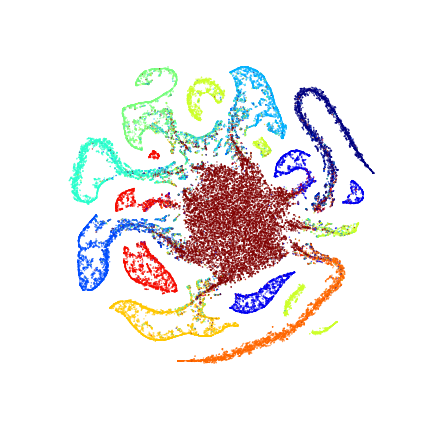
\includegraphics[width=\linewidth]{images/tsne/tsne_ROG_imagenet32.png}
    \caption*{RoG~}
  \end{subfigure}
  \begin{subfigure}{.18\textwidth}
    \centering
    % include second image
    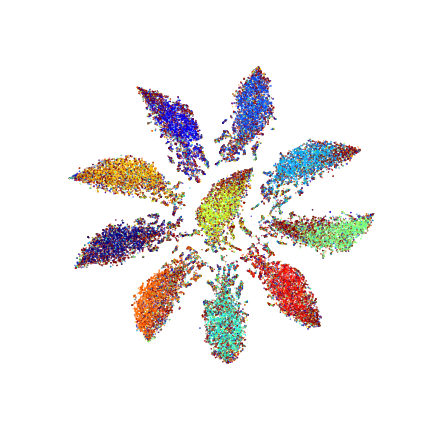
\includegraphics[width=\linewidth]{images/tsne/tsne_ILON_imagenet32.png}
    \caption*{ILON~}
  \end{subfigure}
  \begin{subfigure}{.18\textwidth}
    \centering
    % include second image
   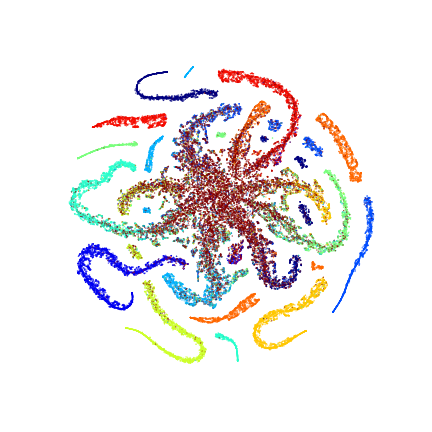
\includegraphics[width=\linewidth]{images/tsne/tsne_ROG_cifar100.png}
   \caption*{RoG~}
  \end{subfigure}
  \begin{subfigure}{.18\textwidth}
    \centering
    % include second image
    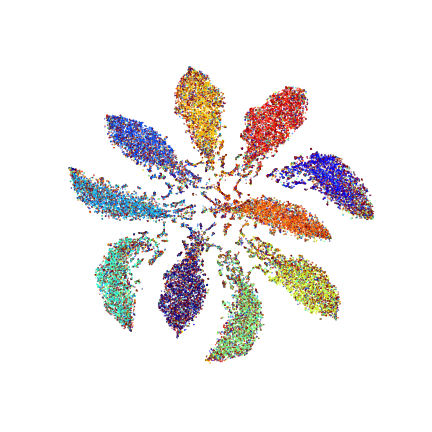
\includegraphics[width=\linewidth]{images/tsne/tsne_ILON_cifar100.png}
    \caption*{ILON~}
  \end{subfigure}
  \\
  \begin{subfigure}{.18\textwidth}
    \centering
    % include first image
    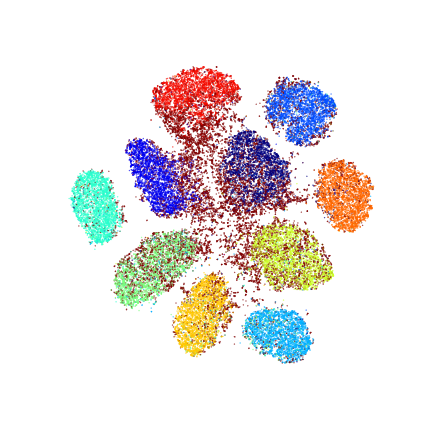
\includegraphics[width=\linewidth]{images/tsne/tsne_DM_imagenet32.png} 
    \caption*{DivideMix~}
  \end{subfigure}
  \begin{subfigure}{.18\textwidth}
    \centering
    % include second image
    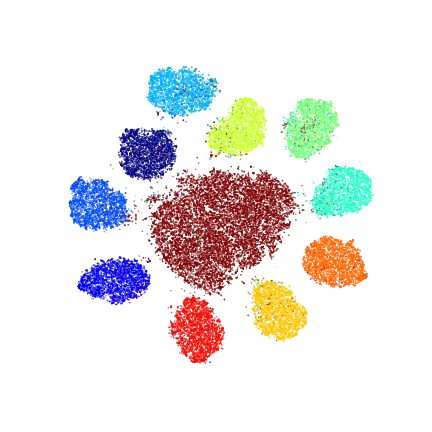
\includegraphics[width=\linewidth]{images/tsne/tsne_EDM_imagenet32_D.png}
    \caption*{EDM [ours]}
  \end{subfigure}
  \begin{subfigure}{.18\textwidth}
    \centering
    % include second image
    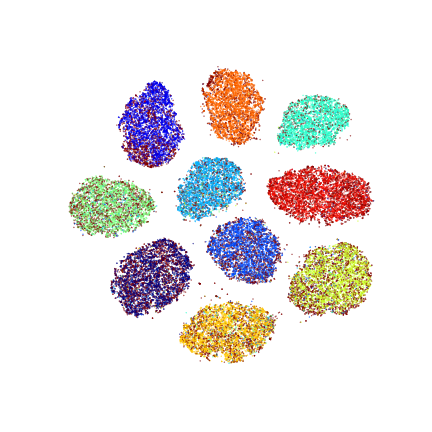
\includegraphics[width=\linewidth]{images/tsne/tsne_DM_cifar100.png}
    \caption*{DivideMix~}
  \end{subfigure}
  \begin{subfigure}{.18\textwidth}
    \centering
    % include second image
    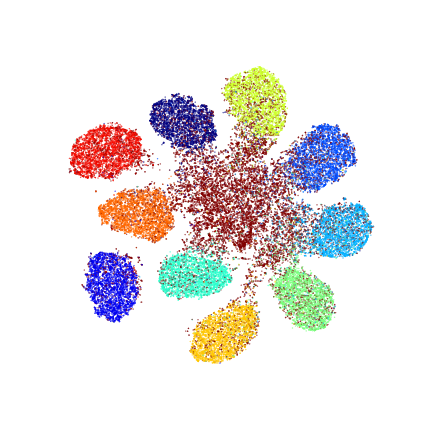
\includegraphics[width=\linewidth]{images/tsne/tsne_EDM_cifar100_D.png}
    \caption*{EDM [ours]}
  \end{subfigure}
  \caption{相关方法和我们提出的EDM方法的TSNE图,其中整体的噪声率是$\rho = 0.6$,
  开集噪声的比率是$\omega = 0.5$,CIFAR-100和ImageNet32表示开集数据集。其中\textbf{棕色}
  样本表示开集噪声样本,其他颜色表示真实的CIFAR-10类别。
  }
  \label{fig4}
\end{figure*}

% 损失分布图
\begin{figure*}[t]
  \centering
  \hspace*{8mm}{\scriptsize EDM [ours] \hspace{50mm} DivideMix }  \\
  \noindent  \rule{5cm}{0.5pt} \hspace{12mm} \rule{5cm}{0.5pt}
  \\
  
  \begin{subfigure}{.18\textwidth}
    \centering
    % include first image
    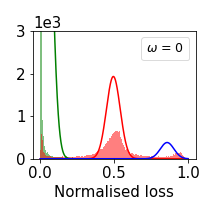
\includegraphics[width=\linewidth]{images/loss_dist/EDM_0.6_1.00_cifar100.png} 
  \end{subfigure}
  \begin{subfigure}{.18\textwidth}
    \centering
    % include second image
    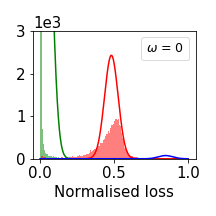
\includegraphics[width=\linewidth]{images/loss_dist/EDM_0.6_1.00_imagenet32.png} 
  \end{subfigure}
  \begin{subfigure}{.18\textwidth}
    \centering
    % include second image
    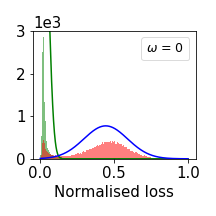
\includegraphics[width=\linewidth]{images/loss_dist/DM_0.6_1.00_cifar100.png} 
  \end{subfigure}
  \begin{subfigure}{.18\textwidth}
    \centering
    % include second image
    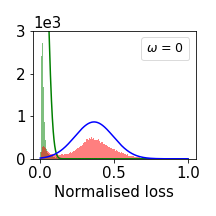
\includegraphics[width=\linewidth]{images/loss_dist/DM_0.6_1.00_imagenet32.png} 
  \end{subfigure}
  \\
  \begin{subfigure}{.18\textwidth}
    \centering
    % include first image
    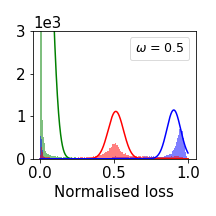
\includegraphics[width=\linewidth]{images/loss_dist/EDM_0.6_0.50_cifar100.png} 
  \end{subfigure}
  \begin{subfigure}{.18\textwidth}
    \centering
    % include second image
    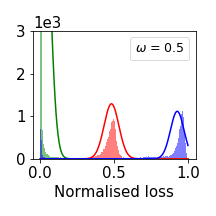
\includegraphics[width=\linewidth]{images/loss_dist/EDM_0.6_0.50_imagenet32.png} 
  \end{subfigure}
  \begin{subfigure}{.18\textwidth}
    \centering
    % include second image
    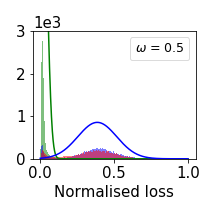
\includegraphics[width=\linewidth]{images/loss_dist/DM_0.6_0.50_cifar100.png} 
  \end{subfigure}
  \begin{subfigure}{.18\textwidth}
    \centering
    % include second image
    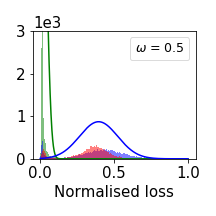
\includegraphics[width=\linewidth]{images/loss_dist/DM_0.6_0.50_imagenet32.png} 
  \end{subfigure}
  \\
  \begin{subfigure}{.18\textwidth}
    \centering
    % include first image
    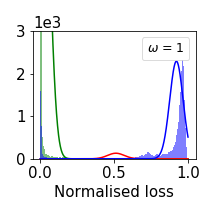
\includegraphics[width=\linewidth]{images/loss_dist/EDM_0.6_0.00_cifar100.png} 
  \end{subfigure}
  \begin{subfigure}{.18\textwidth}
    \centering
    % include second image
    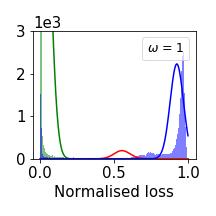
\includegraphics[width=\linewidth]{images/loss_dist/EDM_0.6_0.00_imagenet32.png} 
  \end{subfigure}
  \begin{subfigure}{.18\textwidth}
    \centering
    % include second image
    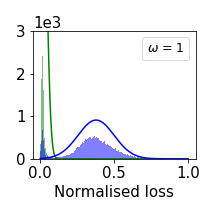
\includegraphics[width=\linewidth]{images/loss_dist/DM_0.6_0.00_cifar100.png} 
  \end{subfigure}
  \begin{subfigure}{.18\textwidth}
    \centering
    % include second image
    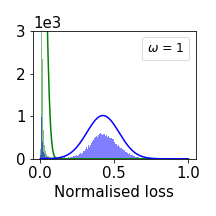
\includegraphics[width=\linewidth]{images/loss_dist/DM_0.6_0.00_imagenet32.png} 
  \end{subfigure}
  \\
  \begin{subfigure}{\textwidth}
    \centering
    % include second image
    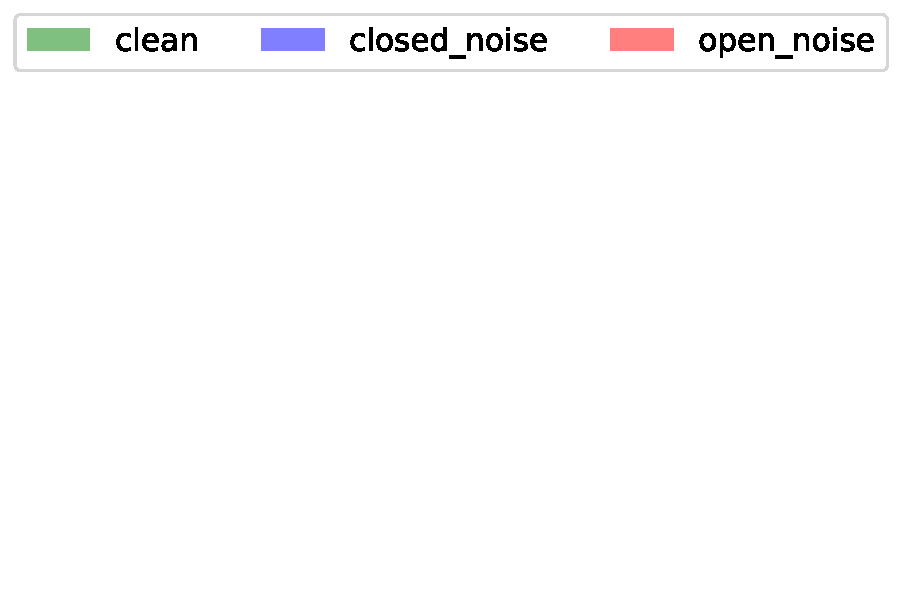
\includegraphics[width=0.4\linewidth]{images/loss_dist/legend.pdf} 
  \end{subfigure}
  \caption{对开集样本(橙色)、闭集样本(蓝色)、干净样本(绿色)的逐样本的loss分布。左边
  由EDM产生,右边由DivideMix产生。周期数为$e=100$,并且$\rho = 0.6$和$\omega  = 0.3$。
  开集噪声样本$\in$\{CIFAR-100,ImageNet32\}。我们同时展示了估计的对干净样本,
  开集样本、闭集样本的GMM后验概率(对于EDM),并展示了使用DivideMix模型时干净样本和噪声
  样本的后验概率分布。}
  \label{fig5}
\end{figure*}


\textbf{噪声分类}:图\ref{fig5}给出了在噪声率$\rho=0.6$,闭集噪声率
为$\omega\in \{0,0.5,1\}$的情况下,干净样本、开集样本和闭集样本
的损失值分布,其中使用来自CIFAR-100和Imagenet32的样本作为开集噪声数据集。
从这些图中可见,显然SL损失能够成功地区分上述三种样本,即使是只有一种噪声类型存在时也是如此
,例如当$\omega \in \{0,1\}$。这表明SL损失在不确定性的识别方面对开集噪声样本是有效的。
本文测试的方法中DivideMix[14]也试图将样本分离成干净样本和噪声样本。然而,结果分布
似乎不足以让三组之间明确分离,因为开集和闭集噪声样本的标签基本上是没有区别的。因此,
DivideMix能够将干净的样本从有噪声的样本中分离出来,而不是将闭集噪声从开集噪声中
分离出来,从而迫使它在训练过程中对这两种噪声类型进行相似的处理(即,两种类型都被视为
闭集噪声)。这是不理想的,因为开放集样本将被分配一个不正确的训练标签,这最终会
导致网络过拟合这些样本。

    
\section{结论}
在本文中,我们研究了一种结合开集[24,13]和闭集噪声[14,13]的标签噪声学习问题的变体。
为了在这个新的问题设定下测试各种方法,我们提出了一个新的基准,系统地改变总噪声率和闭集
与开集噪声的比例。开集样本来自小规模数据集(CIFAR-100)或大规模数据集(ImageNet32),
这样这些样本的真实标签不包含在主要数据集(CIFAR-10)中。我们认为,这样的问题设置更一般,
类似现实生活中的标签噪声场景。然后,我们提出了EvidentialMix算法,成功地解决了这种新
的噪声类型学习问题。我们使用主观逻辑损失[21]产生低损失的干净样本,高损失的闭集噪声样本,
和中等损失的开集样本。训练数据中明确的分工让我们
\textbf{(1)}识别和移除开集噪声样本以避免过度拟合,考虑到他们不属于任何已知的类;
\textbf{(2)}用半监督学习方法从预测的闭集样本[14]中学习。评估表明,我们提出的EDM
方法比目前最先进的闭集问题研究方法[14,13]和开集问题研究方法[24,13]更有效地解决了
这种新的组合开闭集标签噪声学习问题。

\textbf{未来的工作}:引入这个问题的动机是发起研究社区的对话,以研究混合的开集和闭集
标签噪声。接下来,我们将探索更具挑战性的噪声设定,例如将不对称的噪声[19]和语义噪声[13]
合并到提出的组合标签噪声问题中。由于我们是第一个在受控的设定下解决这个问题的,
没有先例说明如何将这些具有挑战性的噪声设定进行有意义的融合。例如,尽管不对称闭集
噪声之前已经在文献[19]中进行了研究,但是它的对等物——不对称开集标签噪声需要什么是不清楚的;
例如,目前还不清楚如何在CIFAR-10和ImageNet类之间建立一个噪声转换矩阵。此外,
我们认为研究其他类型的不确定性来识别开集噪声是有价值的,例如使用贝叶斯学习[4]来识别
。我们也旨在探索这样的方法。

\section{参考文献}
[1] David Berthelot, Nicholas Carlini, Ian Goodfellow, Nicolas
Papernot, Avital Oliver, and Colin Raffel. MixMatch: A
Holistic Approach to Semi-Supervised Learning. arXiv eprints,
page arXiv:1905.02249, May 2019.

[2] Patryk Chrabaszcz, Ilya Loshchilov, and Frank Hutter. A
downsampled variant of imagenet as an alternative to the cifar
datasets. arXiv preprint arXiv:1707.08819, 2017.

[3] Jia Deng, Wei Dong, Richard Socher, Li-Jia Li, Kai Li,
and Li Fei-Fei. Imagenet: A large-scale hierarchical image
database. In 2009 IEEE conference on computer vision and
pattern recognition, pages 248–255. Ieee, 2009.

[4] Yarin Gal and Zoubin Ghahramani. Dropout as a bayesian
approximation: Representing model uncertainty in deep
learning. In international conference on machine learning,
pages 1050–1059, 2016.

[5] Jacob Goldberger and Ehud Ben-Reuven. Training deep
neural-networks using a noise adaptation layer. 2017.

[6] Kaiming He, Xiangyu Zhang, Shaoqing Ren, and Jian Sun.
Identity mappings in deep residual networks. In European
conference on computer vision, pages 630–645. Springer,
2016.

[7] Lu Jiang, Zhengyuan Zhou, Thomas Leung, Li-Jia Li, and
Li Fei-Fei. Mentornet: Learning data-driven curriculum for
very deep neural networks on corrupted labels. In International
Conference on Machine Learning, pages 2304–2313,
2018.

[8] Lance Kaplan, Federico Cerutti, Murat Sensoy, Alun Preece,
and Paul Sullivan. Uncertainty Aware AI ML: Why and
How. arXiv e-prints, page arXiv:1809.07882, Sept. 2018.

[9] Youngdong Kim, Junho Yim, Juseung Yun, and Junmo Kim.
Nlnl: Negative learning for noisy labels. In Proceedings
of the IEEE International Conference on Computer Vision,
pages 101–110, 2019.

[10] Hans-Peter Kriegel, Peer Kr¨oger, Erich Schubert, and Arthur
Zimek. Loop: local outlier probabilities. In Proceedings
of the 18th ACM conference on Information and knowledge
management, pages 1649–1652, 2009.

[11] Alex Krizhevsky, Geoffrey Hinton, et al. Learning multiple
layers of features from tiny images. 2009.

[12] Yann LeCun, Y. Bengio, and Geoffrey Hinton. Deep learning.
Nature, 521:436–44, 05 2015.

[13] Kimin Lee, Sukmin Yun, Kibok Lee, Honglak Lee, Bo Li,
and Jinwoo Shin. Robust inference via generative classifiers
for handling noisy labels. arXiv preprint arXiv:1901.11300,
2019.

[14] Junnan Li, Richard Socher, and Steven C. H. Hoi. DivideMix:
Learning with Noisy Labels as Semi-supervised
Learning. arXiv e-prints, page arXiv:2002.07394, Feb. 2020.

[15] Junnan Li, YongkangWong, Qi Zhao, and Mohan S Kankanhalli.
Learning to learn from noisy labeled data. In Proceedings
of the IEEE Conference on Computer Vision and Pattern
Recognition, pages 5051–5059, 2019.

[16] Laurens van der Maaten and Geoffrey Hinton. Visualizing
data using t-sne. Journal of machine learning research,
9(Nov):2579–2605, 2008.

[17] Eran Malach and Shai Shalev-Shwartz. Decoupling” when
to update” from” how to update”. In Advances in Neural
Information Processing Systems, pages 960–970, 2017.

[18] Giorgio Patrini, Alessandro Rozza, Aditya Krishna Menon,
Richard Nock, and Lizhen Qu. Making deep neural networks
robust to label noise: A loss correction approach. In Proceedings
of the IEEE Conference on Computer Vision and
Pattern Recognition, pages 1944–1952, 2017.

[19] Scott Reed, Honglak Lee, Dragomir Anguelov, Christian
Szegedy, Dumitru Erhan, and Andrew Rabinovich. Training
Deep Neural Networks on Noisy Labels with Bootstrapping.
arXiv e-prints, page arXiv:1412.6596, Dec. 2014.

[20] Mengye Ren, Wenyuan Zeng, Bin Yang, and Raquel Urtasun.
Learning to reweight examples for robust deep learning.
arXiv preprint arXiv:1803.09050, 2018.

[21] Murat Sensoy, Lance Kaplan, and Melih Kandemir. Evidential
deep learning to quantify classification uncertainty, 2018.

[22] Duc Tam Nguyen, Chaithanya Kumar Mummadi, Thi
Phuong Nhung Ngo, Thi Hoai Phuong Nguyen, Laura
Beggel, and Thomas Brox. SELF: Learning to Filter
Noisy Labels with Self-Ensembling. arXiv e-prints, page
arXiv:1910.01842, Oct. 2019.

[23] Antti Tarvainen and Harri Valpola. Mean teachers are better
role models: Weight-averaged consistency targets improve
semi-supervised deep learning results. In Advances in neural
information processing systems, pages 1195–1204, 2017.

[24] Yisen Wang, Weiyang Liu, Xingjun Ma, James Bailey,
Hongyuan Zha, Le Song, and Shu-Tao Xia. Iterative Learning
with Open-set Noisy Labels. arXiv e-prints, page
arXiv:1804.00092, Mar. 2018.

[25] Xingrui Yu, Bo Han, Jiangchao Yao, Gang Niu, Ivor W
Tsang, and Masashi Sugiyama. How does disagreement
help generalization against label corruption? arXiv preprint
arXiv:1901.04215, 2019.

[26] Chiyuan Zhang, Samy Bengio, Moritz Hardt, Benjamin
Recht, and Oriol Vinyals. Understanding deep learning
requires rethinking generalization. arXiv preprint
arXiv:1611.03530, 2016.

[27] Hongyi Zhang, Moustapha Cisse, Yann N Dauphin, and
David Lopez-Paz. mixup: Beyond empirical risk minimization.
arXiv preprint arXiv:1710.09412, 2017.

\end{document}



